\Variant{24.12.2023}
\QQ{1}{Hisoblang:
\[\frac{\text{EKUK}(12;\,6)+\text{EKUB}(6;\,12)}{\sqrt{\text{EKUK}(12;\,3)\cdot\text{EKUB}(3;\,12)}}\]
\Opts{$3$}{$9$}{$6$}{$1$}}
\QQ{2}{Hisoblang:
\[\frac{18}{65}\cdot\left(\frac{41}{18}-\frac{17}{36}\right)+\frac76+\left(\frac47+\frac5{49}\right):\frac{99}{49}\]
\Opts{$\dfrac{16}3$}{$6$}{$2$}{$\dfrac56$}}
\QQ{3}{Oltin va kumuş qotişmasining massasi $1{,}06$ kg. Qotişmani suvga solinganda $70$ gr massasini yöqotadi. Oltin suvda massasining $\dfrac1{19}$ qismini, kumuş esa $\dfrac1{10}$ qismini yöqotadi. Oltin va kumuşning dastlabki massalarini toping.
\Opts{Oltin $760$ gr, kumuş $300$ gr}{Oltin $490$ gr, kumuş $570$ gr}{Oltin $630$ gr, kumuş $430$ gr}{Oltin $570$ gr, kumuş $490$ gr}}
\QQ{4}{Öqişga qabul qiliş uçun $5000$ nafar talabaga kvota ajratilgan. Talabalar sonini oşiriş maqsadida ketma-ket uç yil bir xil foizga qabul kvotasi oşirildi va kvota soni $6655$ taga yetdi. Qabul kvotasi har yili neça foizga oşirilgan?
\Opts{$11$}{$10$}{$12$}{$15$}}
\QQ{5}{Hisoblang:
\[\sqrt{\sqrt{47}-\sqrt{31}}\cdot\sqrt{\sqrt{47}+\sqrt{31}}\]
\Opts{$7$}{$5$}{$6$}{$4$}}
\QQ{6}{$m,n\in\mathbb N$ uçun $3^8\cdot2^{10}\cdot3^{-4}\cdot2^{-4}=2^m\cdot3^n$ bölsa, $m+n$ ni toping.
\Opts{$11$}{$9$}{$10$}{$8$}}
\QQ{7}{Arifmetik progressiyaning birinçi hadi $8$, oxirgi hadi esa $74$ ga teng. Agar arifmetik progressiyaning ayirmasi butun son bölib, u $3$ va $9$ sonlari orasida bölsa, progressiyaning yiğindisini toping.
\Opts{$462$}{$492$}{$512$}{$382$}}
\QQ{8}{$b_n=\dfrac{2^n}{3^{n-1}}$ ketma-ketlikning barça hadlari yiğindisini toping.
\Opts{$6$}{$1$}{$2$}{$3$}}
\QQ{9}{Agar $x>3$ bölsa, $\dfrac{\sqrt{9+6x+x^2}-\sqrt{9-6x+x^2}}{\sqrt{9+6x+x^2}+\sqrt{9-6x+x^2}}$ ni hisoblang.
\Opts{$-\dfrac3x$}{$\dfrac x{\sqrt3}$}{$\dfrac3x$}{$1$}}
\QQ{10}{$\arccos\left(-\dfrac12\right)+\arcsin\left(-\dfrac12\right)$ ni hisoblang.
\Opts{$\dfrac\pi4$}{$\dfrac\pi2$}{$\dfrac\pi3$}{$1$}}
\QQ{11}{Ifodani soddalaştiring:
\[\frac{2\cos^22\alpha+\cos6\alpha-1}{0{,}5\sin6\alpha+\sin2\alpha\cos2\alpha}\]
\Opts{$2\ctg5\alpha$}{$2\tg5\alpha$}{$\ctg5\alpha$}{$\tg5\alpha$}}
\QQ{12}{Soddalaştiring:
\[\frac{r^2+5r}{r^3-27}-\frac{2r-9}{r^3-27}\]
\Opts{$\dfrac1{3-r}$}{$\dfrac1{r+3}$}{$\dfrac r{r-3}$}{$\dfrac1{r-3}$}}
\QQ{13}{Agar $2^a=5$, $2^b=3$ bölsa, $\left(\dfrac{25}3\right)^c=405$ tenglikdan foydalanib $c$ ni $a$ va $b$ orqali ifodalang.
\Opts{$\dfrac{b+4a}{2a-b}$}{$\dfrac{4b+a}{2a+b}$}{$\dfrac{4b+a}{2a-b}$}{$\dfrac{4b-a}{2a-b}$}}
\QQ{14}{$x^2-6|x|+5\le0$ tengsizlikni qanoatlantiradigan butun sonlar neçta?
\Opts{$8$}{$9$}{$10$}{$11$}}
\QQ{15}{$5^{\frac x{x-3}}-5\cdot5^{\frac3{x-3}}=0$ tenglamaning neçta haqiqiy ildizi bor?
\Opts{$0$}{$1$}{$2$}{Çeksiz köp}}
\QQ{16}{$2x^2-4x-6=0$ tenglama ildizlari yiğindisini toping.
\Opts{$-4$}{$2$}{$4$}{$-2$}}
\QQ{17}{Tenglama ildizlari köpaytmasini toping.
\[\left(\frac1{\sqrt{3+2\sqrt2}}\right)^x+\left(\frac1{\sqrt{3-2\sqrt2}}\right)^x=6\]
\Opts{$-4$}{$4$}{$-2$}{$2$}}
\QQ{18}{Tengsizlikning natural yeçimlari neçta?
\[\frac{25-4x}{\sqrt[3]{10}-2}\ge0\]
\Opts{$10$}{$4$}{$8$}{$6$}}
\QQ{19}{$\sqrt{\log_3\left(36-12x+x^2\right)^8}+6\log_9\sqrt{18-3x}=7$ tenglamaning ildizlari yiğindisini toping.
\Opts{$-3$}{$3$}{$17$}{$-7$}}
\QQ{20}{Quyidagi funksiyalardan neçtasi toq ham, juft ham emas?
\[\text{a) } \frac{x^4+x^2+1}{(x+1)^2+1}\qquad \text{b) } \frac{x\sin x}{x^2+1}\qquad \text{c) } \frac{\cos x}{x+\tg x}\qquad \text{d) } \frac{(x+1)^3+1}{\sin x+x}\]
\Opts{$1$}{$2$}{$3$}{$4$}}
\QQ{21}{Funksiyaning eng kiçik musbat davrini toping:
\[f(x)=2\cos^2x+\sin\frac x2+\tg\frac x3\]
\Opts{$12\pi$}{$6\pi$}{$4\pi$}{$9\pi$}}
\QQ{22}{$f(x)=\dfrac1{x^2+3}$ funksiyaning $(1;\,0)$ nuqtadan ötuvçi boşlanğiç funksiyasini toping.
\Opts{$F(x)=\dfrac3{\sqrt3}\left(\arctg\dfrac x{\sqrt3}-\dfrac\pi6\right)$}{$F(x)=\dfrac1{3\sqrt3}\left(\arctg\dfrac x{\sqrt3}+\dfrac\pi6\right)$}{$F(x)=\dfrac1{\sqrt3}\left(\arctg\dfrac x{\sqrt3}-\dfrac\pi6\right)$}{$F(x)=\dfrac{\sqrt3}3\left(\arctg\dfrac x{\sqrt3}+\dfrac\pi6\right)$}}
\QQ{23}{$f(x)=\left|x-\sin^2x-\cos x\right|$ funksiyaning $x_0=\dfrac\pi3$ nuqtadagi hosilasini toping.
\Opts{$-1$}{$1$}{$0$}{Mavjud emas}}
\QQ{24}{Aylana uzunligi $12$ cm, uzunligi $3$ cm bölgan yoyning burçak ölçovini toping.
\Opts{$\dfrac\pi8$}{$\dfrac\pi2$}{$\dfrac{4\pi}6$}{$\dfrac{5\pi}6$}}
\QQ{25}{Rasmda $AB\parallel ED$ bölsa, $x$ burçak qiymatini toping.
\qfig{\begin{tikzpicture}[scale=0.85,font=\small]
\coordinate (B) at (0,0); \coordinate (C) at (5,0); \coordinate (A) at (2.038,3.53); \coordinate (D) at (2.482,3.0); \coordinate (E) at (-0.018,-1.33); \coordinate (F) at (4.338,-2.098);
\draw (A)--(B)--(C)--cycle; \draw (D)--(E)--(F)--cycle;
\draw (0.45,0) arc (0:60:0.45); \node at (0.75,0.32) {\scriptsize$60^\circ$};
\draw (4.55,0) arc (180:130:0.45); \node at (4.15,0.3) {\scriptsize$50^\circ$};
\draw ($(E)!0.4cm!(D)$) arc (60:-10:0.4cm); \node at (0.55,-0.75) {\scriptsize$70^\circ$};
\draw ($(F)!0.4cm!(E)$) arc (170:110:0.4cm); \node at (3.55,-1.6) {\scriptsize$60^\circ$};
\draw ($(D)!0.45cm!(F)$) arc (290:310:0.45cm); \node at (2.68,2.35) {\scriptsize$x$};
\node[above] at (A) {$A$}; \node[left] at (B) {$B$}; \node[right] at (C) {$C$}; \node[above right] at (D) {$D$}; \node[left] at (E) {$E$}; \node[below right] at (F) {$F$};
\end{tikzpicture}}
\Opts{$50^\circ$}{$30^\circ$}{$35^\circ$}{$20^\circ$}}
\QQ{26}{Quyidagi çizmada $ABCDE$ muntazam beşburçak berilgan, $CD=DK$, $CD\perp DK$, $K$ nuqta $FE$ kesmada yotadi. Bunga köra $\alpha$ burçak qiymatini toping.
\qfig{\begin{tikzpicture}[scale=2.1,font=\small]
\coordinate (C) at (0,1); \coordinate (D) at (0.951,0.309); \coordinate (E) at (0.588,-0.809); \coordinate (A) at (-0.588,-0.809); \coordinate (B) at (-0.951,0.309); \coordinate (K) at (0.26,-0.642); \coordinate (F) at (-0.821,-0.091);
\draw (A)--(B)--(C)--(D)--(E)--cycle; \draw (C)--(K)--(D); \draw (F)--(E);
\draw ($(D)!0.12!(C)$)--($(D)!0.12!(C)!0.12!-90:(C)$)--($(D)!0.12!(K)$);
\draw ($(C)!0.5!(D)+(-0.04,-0.05)$)--++(0.08,0.1); \draw ($(K)!0.5!(D)+(-0.06,0.03)$)--++(0.12,-0.06);
\draw ($(F)!0.2cm!(E)$) arc (-27:-72:0.2cm); \node at ($(F)+(0.22,-0.26)$) {\scriptsize$\alpha$};
\node[above] at (C) {$C$}; \node[right] at (D) {$D$}; \node[below right] at (E) {$E$}; \node[below left] at (A) {$A$}; \node[left] at (B) {$B$}; \node[left] at (F) {$F$}; \node[below] at (K) {$K$};
\end{tikzpicture}}
\Opts{$45^\circ$}{$55^\circ$}{$35^\circ$}{$40^\circ$}}
\QQ{27}{$ABC$ uçburçakning yuzi $60$ ga, $\overrightarrow{BE}=-\dfrac12\overrightarrow{BA}$ bölsa, $BEC$ uçburçak yuzini toping.
\Opts{$60$}{$120$}{$30$}{$90$}}
\QQ{28}{$ABC$ teng yonli ($AB=AC$) uçburçakka aylana içki çizilgan va yon tomonini uriniş nuqtasidan $2$ va $5$ ga teng kesmalarga ajratgan bölib, $AB<BC$ bölsa, uçburçak yuzini toping.
\Opts{$10\sqrt3$}{$5\sqrt6$}{$5\sqrt3$}{$10\sqrt6$}}
\QQ{29}{$ABCD$ töğri burçakli trapetsiyaning asoslari $BC=8$ va $AD=24$ ga teng bölsa, diagonallar kesişgan nuqtadan kiçik yon tomonigaça bölgan eng qisqa masofani toping.
\Opts{$3$}{$6$}{$4{,}5$}{$5{,}8$}}
\QQ{30}{Tekislikda yotmagan $O$ nuqtadan tekislikka ikkita $OA$ va $OB$ oğmalar tuşirilgan. $OA$ oğmaning uzunligi $OB$ oğmaning uzunligidan $14$ ga ortiq. Ularning proyeksiyalari mos ravişda $36$ va $20$ bölsa, $O$ nuqtadan tekislikkaça bölgan eng qisqa masofani toping.
\Opts{$25$}{$20$}{$15$}{$12$}}
\QQ{31}{$A=\{x\mid-3\le x\le2,\ x\in\mathbb Z\}$, $B=\{x\mid-1<x<3,\ x\in\mathbb N\}$, $C=\{x\mid-3\le x<1,\ x\in\mathbb Z\}$ berilgan. $(A\cap B)\cup C$ ning elementlar sonini toping.
\Opts{$13$}{$7$}{$6$}{$4$}}
\QQ{32}{Barça raqamlari $5$ dan katta bölmagan, raqamlari takrorlanmaydigan $3$ xonali sonlar neçta?
\Opts{$125$}{$120$}{$80$}{$100$}}
\QQ{33}{\Moslash{Hajmi $V_p=6\left(\sqrt7+1\right)^3$ bölgan muntazam törtburçakli piramidaga şar içki çizilgan. Yon qirrasi va asos tekisligi orasidagi burçak $60^\circ$ ga teng. Şarga oktaedr (muntazam $8$ yoqli) içki çizilgan. ($\pi\approx3$ deb oling.)
\par\centering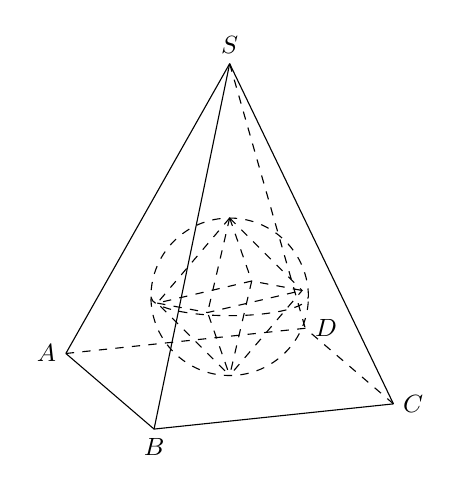
\begin{tikzpicture}[scale=0.8,font=\small]
\coordinate (A) at (-2.6,0.4); \coordinate (B) at (-1.2,-0.8); \coordinate (C) at (2.6,-0.4); \coordinate (D) at (1.2,0.8); \coordinate (S) at (0,5);
\draw (A)--(B)--(C); \draw[dashed] (A)--(D)--(C); \draw (S)--(A); \draw (S)--(B); \draw (S)--(C); \draw[dashed] (S)--(D);
\draw[dashed] (0,1.3) circle (1.25); \draw[dashed] (-1.25,1.3) arc (180:360:1.25 and 0.3);
\coordinate (T) at (0,2.55); \coordinate (U) at (0,0.05); \coordinate (P1) at (-1.15,1.2); \coordinate (P2) at (-0.35,1.05); \coordinate (P3) at (1.15,1.4); \coordinate (P4) at (0.35,1.55);
\draw[dashed] (P1)--(P2)--(P3)--(P4)--cycle; \foreach \p in {P1,P2,P3,P4} {\draw[dashed] (T)--(\p)--(U);}
\node[left] at (A) {$A$}; \node[below] at (B) {$B$}; \node[right] at (C) {$C$}; \node[right] at (D) {$D$}; \node[above] at (S) {$S$};
\end{tikzpicture}}{A) $36$\par B) $18$\par C) $108$\par D) $54$\par E) $36\sqrt3$\par F) $18\sqrt3$}{Şar sirtining yuzini toping.}{Oktaedr sirtining yuzini toping.}{Oktaedr hajmini toping.}}
\QQ{36}{Tenglamalar sistemasi berilgan.
\[\begin{cases}2|x-5|-y+6=0,\\ |2y-3|-6x-5=0\end{cases}\]
\AB{Tenglamalar sistemasini qanoatlantiruvçi neçta $(x;y)$ haqiqiy sonlar juftligi bor?}{Barça $x$ va $y$ lar yiğindisini toping.}}
\QQ{37}{$\sin\left(\dfrac{2\pi}3\cos3x\right)=\dfrac{\sqrt3}2$ tenglama berilgan.
\AB{Tenglamaning eng katta manfiy yeçimini toping.}{$\left[-\dfrac{5\pi}3;\ \dfrac{2\pi}3\right]$ oraliqdagi yeçimlari neçta?}}
\QQ{38}{$f(g(x))=\dfrac{\sqrt{1-x^2}}2$ va $g(x)=2x+1$ funksiyalar berilgan.
\AB{$f(x)$ ning aniqlaniş sohasini toping.}{$f(x)$ ning qiymatlar sohasini toping.}}
\QQ{39}{$y=ax^2+bx+c$ funksiya grafigi berilgan. Funksiya $x_0=2$ nuqtada eng katta qiymatga erişadi.
\qfig{\begin{tikzpicture}[x=0.3cm,y=0.42cm,font=\small]
\draw[-{Stealth[length=4pt]}] (-6.5,0)--(10.5,0) node[right] {$x$}; \draw[-{Stealth[length=4pt]}] (0,-4.2)--(0,7.2) node[left] {$y$};
\draw[thick,domain=-5.6:9.6,samples=60] plot (\x,{-5/32*(\x+4)*(\x-8)});
\draw[dashed] (2,0)--(2,5.625); \node[below left] at (-4,0) {$-4$}; \node[below] at (2,0) {$2$}; \node[below right] at (8,0) {$8$}; \node[left] at (0,5.3) {$5$};
\end{tikzpicture}}
\AB{$x$ ning $[-6;\,9]$ oraliqdagi qaysi qiymatida $f'(x)$ funksiya eng katta qiymatga erişadi?}{$[-6;\,9]$ kesmada $f(x)\cdot f'(x)\le0$ tengsizlikning neçta butun yeçimi bor?}}
\QQ{40}{Çizmada $f(x)=\sqrt{x+a+b}$ funksiya grafigining $[1;\,5]$ kesmadagi qismi tasvirlangan.
\qfig{\begin{tikzpicture}[x=0.7cm,y=0.7cm,font=\small]
\draw[-{Stealth[length=4pt]}] (-0.6,0)--(6.5,0) node[right] {$x$}; \draw[-{Stealth[length=4pt]}] (0,-0.6)--(0,2.8) node[left] {$y$};
\draw[thick,domain=1:5,samples=60] plot (\x,{sqrt(\x-1)});
\draw[dashed] (0,2)--(5,2)--(5,0); \node[below] at (1,0) {$1$}; \node[below] at (5,0) {$5$}; \node[left] at (0,2) {$2$};
\end{tikzpicture}}
\AB{$a+b$ ni toping.}{$x\in[1;\,5]$ oraliqda $f(x)$ funksiyani $Ox$ öqi atrofida $360^\circ$ ga aylantirişdan hosil bölgan jism hajmini toping ($\pi\approx3$ deb oling).}}
\QQ{41}{$ABC$ uçburçakda $AB=5$, $BC=7$ va $AC=9$. Uning $AC$ tomonidan olingan $M$ nuqtadan uçburçakning $AB$ va $BC$ tomonlarigaça bölgan eng qisqa masofalar teng.
\qfig{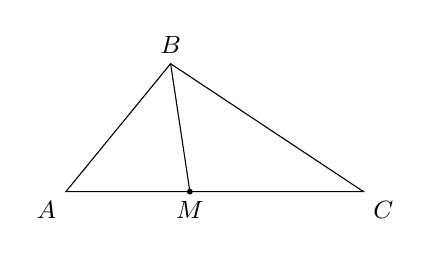
\begin{tikzpicture}[scale=0.42,font=\small]
\coordinate (A) at (0,0); \coordinate (C) at (9,0); \coordinate (B) at (3.167,3.869); \coordinate (M) at (3.75,0);
\draw (A)--(B)--(C)--cycle; \draw (B)--(M); \fill (M) circle (2.5pt);
\node[below left] at (A) {$A$}; \node[above] at (B) {$B$}; \node[below right] at (C) {$C$}; \node[below] at (M) {$M$};
\end{tikzpicture}}
\AB{$M$ nuqtadan $AB$ tomongaça bölgan eng qisqa masofani toping.}{$|MC|-|MA|$ ayirmani toping.}}
\QQ{42}{Radiusi $3\sqrt6$ ga teng bölgan şarga eng katta hajmli konus içki çizilgan. ($\pi\approx3$ deb oling.)
\qfig{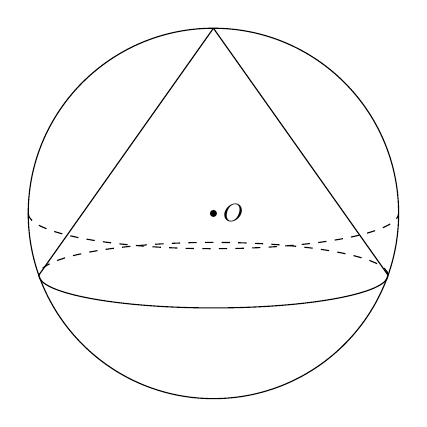
\begin{tikzpicture}[scale=0.32,font=\small]
\draw (0,0) circle (7.35); \draw (-6.93,-2.45) arc (180:360:6.93 and 1.3); \draw[dashed] (6.93,-2.45) arc (0:180:6.93 and 1.3);
\draw (0,7.35)--(-6.93,-2.45); \draw (0,7.35)--(6.93,-2.45); \draw[dashed] (-7.35,0) arc (180:360:7.35 and 1.4);
\fill (0,0) circle (4pt); \node[right] at (0,0) {$O$};
\end{tikzpicture}}
\AB{Konusning yasovçisini toping.}{Konus hajmini toping.}}
\QQ{43}{Rasmda kiçik asosi $5$ ga, balandligi $4$ ga bölgan teng yonli $ABCD$ trapetsiyada $\cos\angle ABD=-\dfrac2{5\sqrt5}$, $\cos\angle CDB=\dfrac2{\sqrt5}$ berilgan. $E$ va $F$ — mos ravişda $AC$ va $BD$ diagonallarning örtalari.
\qfig{\begin{tikzpicture}[scale=0.62,font=\small]
\coordinate (A) at (0,0); \coordinate (D) at (11,0); \coordinate (B) at (3,4); \coordinate (C) at (8,4); \coordinate (E) at (4,2); \coordinate (F) at (7,2);
\draw (A)--(B)--(C)--(D)--cycle; \draw (A)--(C); \draw (B)--(D); \draw (E)--(F); \fill (E) circle (2.5pt); \fill (F) circle (2.5pt);
\draw ($(B)!0.6cm!(A)$) arc (233.13:333.43:0.6cm); \draw ($(D)!0.7cm!(C)$) arc (126.87:153.43:0.7cm);
\node[below left] at (A) {$A$}; \node[below right] at (D) {$D$}; \node[above left] at (B) {$B$}; \node[above right] at (C) {$C$}; \node[above] at (5.5,4) {$5$};
\node[below] at (E) {$E$}; \node[below] at (F) {$F$};
\end{tikzpicture}}
\AB{Diagonallar örtalarini tutaştiruvçi $EF$ kesma uzunligini toping.}{Trapetsiya yuzini toping.}}
\QQ{44}{Rasmda markazlari $A$, $B$, $C$, $D$, $E$ bölgan $5$ ta aylana berilgan, qöşni aylanalar özaro taşqi urinadi. Bunda $AB=15$, $BC=14$, $CD=12$, $DE=10$, $AE=11$.
\qfig{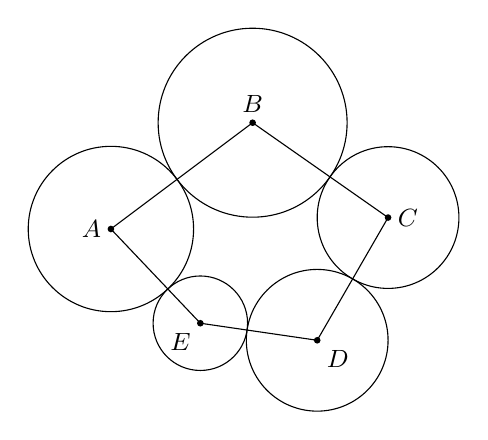
\begin{tikzpicture}[scale=0.15,font=\small]
\coordinate (A) at (0,0); \coordinate (B) at (12,9); \coordinate (C) at (23.468,0.97); \coordinate (D) at (17.468,-9.422); \coordinate (E) at (7.573,-7.978);
\draw (A) circle (7); \draw (B) circle (8); \draw (C) circle (6); \draw (D) circle (6); \draw (E) circle (4);
\draw (A)--(B)--(C)--(D)--(E)--cycle; \foreach \p in {A,B,C,D,E} \fill (\p) circle (8pt);
\node[left] at (A) {$A$}; \node[above] at (B) {$B$}; \node[right] at (C) {$C$}; \node[below right] at (D) {$D$}; \node[below left] at (E) {$E$};
\end{tikzpicture}}
\AB{$E$ markazli aylana uzunligini toping ($\pi\approx3$ deb oling).}{Markazi $C$ nuqtada bölgan aylana bilan çegaralangan soha yuzini toping ($\pi\approx3$ deb oling).}}
\QQ{45}{Uyning tomiga eni $36$ cm, uzunligi $15$ m bölgan tunukadan eng katta siğimli tarnov örnatilgan. Tarnov balandligi $x$ cm dan iborat.
\qfig{\begin{tikzpicture}[scale=0.9,font=\small]
\coordinate (P1) at (0,1); \coordinate (P2) at (0,0); \coordinate (P3) at (2,0); \coordinate (P4) at (2,1); \coordinate (v) at (5,2.5);
\fill[qfill!45] (P1)--(P2)--($(P2)+(v)$)--($(P1)+(v)$)--cycle; \fill[qfill!70] (P2)--(P3)--($(P3)+(v)$)--($(P2)+(v)$)--cycle; \fill[qfill] (P3)--(P4)--($(P4)+(v)$)--($(P3)+(v)$)--cycle;
\draw (P1)--(P2)--(P3)--(P4); \draw (P1)--($(P1)+(v)$)--($(P2)+(v)$); \draw (P2)--($(P2)+(v)$)--($(P3)+(v)$); \draw (P3)--($(P3)+(v)$)--($(P4)+(v)$)--(P4);
\node[left] at (0,0.5) {$x$}; \node[below] at (1,0) {$36-2x$}; \node[below right] at (4.5,1.25) {$15$\,m};
\end{tikzpicture}}
\AB{Tarnov balandligini $x$ (cm) toping.}{Tarnov siğimi neça litrga teng?}}
\Javoblar{A C A B D C B A C B A D C C D B A D B B A C A B D A C D B C C D C E A}{\OK{36}{$1$}{$13{,}6$}\OK{37}{$-\dfrac\pi9$}{$11$}\OK{38}{$[-1;\,3]$}{$[0;\,0{,}5]$}\OK{39}{$-6$}{$10$}\OK{40}{$-1$}{$24$}\OK{41}{$\dfrac{7\sqrt{11}}8$}{$1{,}5$}\OK{42}{$12$}{$192\sqrt6$}\OK{43}{$3$}{$32$}\OK{44}{$24$}{$108$}\OK{45}{$9$}{$243$}}
